\documentclass[a4paper,12pt]{article}

\sloppy
\frenchspacing

\usepackage[left=4cm,top=4cm,right=4cm,bottom=4cm,nohead]{geometry}
\usepackage[utf8]{inputenc}
\usepackage[magyar]{babel}
\usepackage{listings}
\usepackage{multicol}
\usepackage{graphicx}
\usepackage{makecell}
\usepackage{float}

\title{Szoftverarchitektúrák (VIAUM105)\\Egyszerű verziókövető rendszer\\Felhasználói dokumentáció}
\author{Vajna Miklós (AYU9RZ)\\Veres-Szentkirályi András (YZIOAW)}

\begin{document}

\maketitle
\thispagestyle{empty}
\lstset{numbers=left, numberstyle=\tiny, basicstyle=\ttfamily, breaklines=true, frame=single, tabsize=2}

\pagebreak
\onehalfspacing
\section{Bevezetés}

A felhasználói dokumentáció célja, hogy bemutassa a felhasználó számára mind a
szerver, mind a kliens alkalmazás használatát, amennyiben annak telepítése
már a telepítési útmutató szerint megtörtént.

\section{A szerver használata}

A szerver komponens nem rendelkezik grafikus felhasználói felülettel: a kezdeti
beállításokat parancssoros interfészen keresztül lehet beállítani, majd később
a már beállított értékeket újra felhasználva nem-interaktív módban is
indítható. A szerver a következő parancssori kapcsolókkal rendelkezik:

\begin{center}
\begin{table}[H]
\centering
\begin{tabular}{| l | l | l |}
\hline
Név & Funkció & Típus \\ \hline
-ORBendPoint \emph{érték} & \makecell[l]{CORBA végpont \\ megadása, például \\ 31337-es  TCP \\ port esetén\\ giop:tcp::31337} & kötelező \\
\hline
\makecell[l]{-ORBnativeCharCodeSet \\ \emph{érték}} & \makecell[l]{CORBA karakterkódolás \\ megadása, például \\ UTF-8} & kötelező \\
\hline
-yes & \makecell[l]{korábban elmentett \\ beállítások használata, \\ interaktív mód \\ tiltása} & opcionális \\
\hline
\end{tabular}
\caption{A szerver elérhető kapcsolói}
\end{table}
\end{center}

A szervert bináris formában csak Linux rendszerre tettük elérhetővé, ott az
sql-version-control-server parancs indítja.

Interaktív mód esetén indításkor a szerver a következő paraméterekre kérdez rá:

\begin{itemize}
\item MySQL host neve
\item MySQL adatbázis neve
\item MySQL felhasználó neve
\item MySQL felhasználó jelszava
\end{itemize}

A MySQL felhasználó jelszavát a szerver soha nem tárolja le biztonsági okokból,
így ha nem-interaktív módban szeretnénk használni a szervert, állítsuk be a
MySQL hozzáférést az adott felhasználóra és elérési hostra jelszó nélkül
engedélyezettre.

\section{A kliens használata}

A kliens elérhető mind Linux, mind Windows rendszeren, indításához:

\begin{itemize}
\item Linuxon adjuk ki az sql-version-control-gui parancsot
\item Windowson válasszuk a Start menüből az SQL Version Control elemet
\end{itemize}

A kliens indulásakor meg kell adjuk a szerver elérhetőségét, valamint
felhasználói nevünket és jelszavunkat:

\begin{figure}[H]
\centering
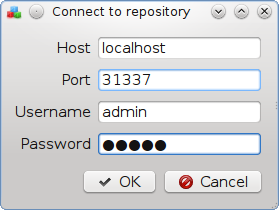
\includegraphics[width=50mm,keepaspectratio]{user-login.png}
\caption{Bejelentkezés}
\end{figure}

Ezután a klienst mind adminisztrációhoz, mind az SQL scriptek verzióinak
kezeléséhez használhatjuk.

\subsection{A kliens használata adminisztrációhoz}

A kliens adminisztrációs felületet biztosít felhasználók létrehozásához, azok
adatainak módosításához valamint törlésükhöz.

Felhasználó létrehozásához válasszuk az Administration / Manage users
menüpontot, majd kattintsunk az Add gombra. Ezt követően adjuk meg a
felhasználó nevét és kattintsunk az OK gombra:

\begin{figure}[H]
\centering
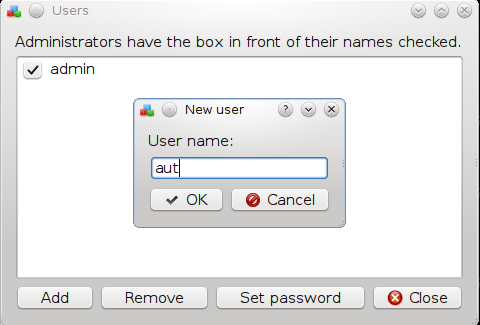
\includegraphics[width=100mm,keepaspectratio]{user-create.png}
\caption{Felhasználó létrehozása}
\end{figure}

A felhasználó jelszavának beállításához ezután használjuk a Set password
gombot, adjuk meg az új jelszót, végül kattintsunk az OK gombra:

\begin{figure}[H]
\centering
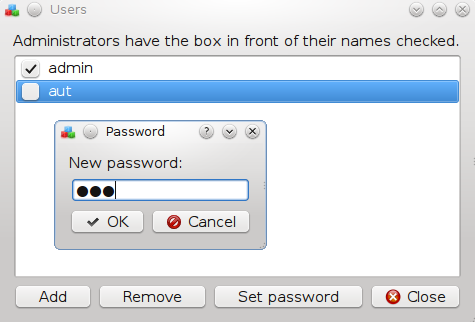
\includegraphics[width=100mm,keepaspectratio]{user-passwd.png}
\caption{Felhasználó létrehozása}
\end{figure}

Ha a felhasználónak adminisztratív jogokat is kívánunk biztosítani, használjuk
a felhasználó neve mellett elérhető jelölőnégyzetet.

Felhasználók törléséhez válasszuk ki a törlendő felhasználót, kattintsunk a
Remove gombra, majd erősítsük meg szándékunkat:

\begin{figure}[H]
\centering
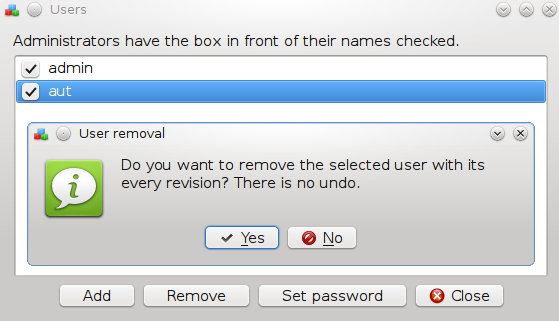
\includegraphics[width=100mm,keepaspectratio]{user-delete.png}
\caption{Felhasználó létrehozása}
\end{figure}

\subsection{A kliens használata a verziók kezeléséhez}

Az SQL scriptek verzióinak kezeléséhez szükséges funkciók használatát ismerteti
ez a szakasz. Az SQL scriptek adatbázis sémákat modelleznek, így a továbbiakban
a scripteket leíró objektumokat modellnek nevezzük.

A modelleknek a következő operációit támogatja a rendszer:

\begin{itemize}
\item modell létrehozása
\item adott verzió mentése külső file-ba
\item új verzió hozzáadása külső file-ból
\item modell törlése
\item modell zárolása, ill. annak megszüntetése
\item modell verzióinak listázása
\end{itemize}

A továbbiakban ezen funkciók használatát ismertetjük.

\subsubsection{Modell létrehozása}

Új modell létrehozására azért van szükségünk, hogy azt követően a modellnek egy
verzióját létre tudjuk hozni, majd a többi felhasználóval kollaborálni tudjunk.

Első lépésben a tényleges modellt kell létrehozni, annak nevének megadásával,
az Administration / New model menüpontot választva:

\begin{figure}[H]
\centering
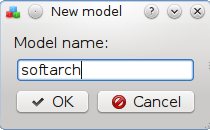
\includegraphics[width=50mm,keepaspectratio]{model-create.png}
\caption{Modell létrehozása}
\end{figure}

Ezt követően az Administration / Edit ACL menüpontot választva adhatunk a
nem-adminisztrátor felhasználóknak olvasás vagy írás jogot a modellhez.

\subsubsection{Modell commitolása}

A modell kezdetben üres, tehát nem tartalmaz verziókat. A commit művelet arra
szolgál, hogy új verziót adjunk a modellhez. Ezt úgy tehetjük meg, hogy egy
külső file-ban elkészítjük a modellt, majd a Modell / Commit menüpontot
használva importáljuk a file-t a programba.

\subsubsection{Modell letöltése}
\subsubsection{Modell törlése}
\subsubsection{Modell zárolása}

\end{document}
